
\documentclass[reqno,11pt]{amsart}

%\usepackage{color,graphicx}
%\usepackage{mathrsfs,amsbsy}
\usepackage{amssymb}
\usepackage{amsmath}
\usepackage{amsfonts}
\usepackage{bm}
\usepackage{graphicx}
\usepackage{amsthm}
\usepackage{enumerate}
\usepackage[mathscr]{eucal}
\usepackage{float}
\usepackage{mathrsfs}
\usepackage{multicol}
\usepackage{multirow}
\usepackage[all,pdf]{xy}
\usepackage[a4paper,left=3cm,right=3cm]{geometry}
\usepackage[table,xcdraw]{xcolor} % before tikz-cd
\usepackage{tikz-cd}
\usepackage{quiver} 
\usepackage{resizegather}
%\usepackage[notcite,notref]{showkeys}

% showkeys  make label explicit on the paper

\makeatletter
\@namedef{subjclassname@2010}{%
  \textup{2010} Mathematics Subject Classification}
\makeatother

\numberwithin{equation}{section}

\theoremstyle{plain}
\newtheorem{theorem}{Theorem}[section]
\newtheorem{lemma}[theorem]{Lemma}
\newtheorem{proposition}[theorem]{Proposition}
\newtheorem{corollary}[theorem]{Corollary}
\newtheorem{claim}[theorem]{Claim}
\newtheorem{defn}[theorem]{Definition}
\newtheorem{ques}[theorem]{Question}
\newtheorem*{fact}{Facts}
\newtheorem{eg}[theorem]{Example}
\newtheorem*{notation}{Conventions and Notations}

\theoremstyle{plain}
\newtheorem{thmsub}{Theorem}[subsection]
\newtheorem{lemmasub}[thmsub]{Lemma}
\newtheorem{corollarysub}[thmsub]{Corollary}
\newtheorem{propositionsub}[thmsub]{Proposition}
\newtheorem{defnsub}[thmsub]{Definition}

\numberwithin{equation}{section}


\theoremstyle{remark}

\newtheorem{remark}[theorem]{Remark}
\newtheorem{remarks}{Remarks}

%\renewcommand\thefootnote{\fnsymbol{footnote}}
%dont use number as footnote symbol, use this command to change

\DeclareMathOperator{\supp}{supp}
\DeclareMathOperator{\dist}{dist}
\DeclareMathOperator{\vol}{vol}
\DeclareMathOperator{\diag}{diag}
\DeclareMathOperator{\tr}{tr}
\DeclareMathOperator{\Img}{\operatorname{Im}}
\DeclareMathOperator{\Id}{\operatorname{Id}}
\DeclareMathOperator{\Rep}{\operatorname{Rep}}
\DeclareMathOperator{\Mod}{\operatorname{mod}}
\DeclareMathOperator{\Hom}{\operatorname{Hom}}
\DeclareMathOperator{\Ext}{\operatorname{Ext}}
\DeclareMathOperator{\gldim}{\operatorname{gl.dim}}
\DeclareMathOperator{\projdim}{\operatorname{proj.dim}}
\DeclareMathOperator{\injdim}{\operatorname{inj.dim}}
\DeclareMathOperator{\dimv}{\operatorname{\underline{\mathbf{dim}}}}


\DeclareMathOperator{\Flagd}{\operatorname{Flag}_{d}}
\DeclareMathOperator{\Flagdstr}{\operatorname{Flag}_{d,str}}
\newcommand{\Gr}{\operatorname{Gr}}
\newcommand{\Grr}{\operatorname{Gr}}
\newcommand{\Gralg}[1]{\operatorname{Gr}^{#1}}
\newcommand{\Grq}{\operatorname{Gr}^{KQ}}
\newcommand{\Flag}[1]{\operatorname{Flag}_{#1}}
\newcommand{\Flagstr}[1]{\operatorname{Flag}_{#1,str}}
\newcommand{\dimvec}[1]{\boldsymbol{#1}}
\newcommand{\ord}{\operatorname{ord}}
\newcommand{\orde}{\operatorname{ord}_e }
\newcommand{\representation}[2]{\genfrac{}{}{0pt}{3}{\phantom{000}#2\phantom{00}}{#1}}
%https://tex.stackexchange.com/questions/96549/how-do-i-write-above-a-left-right-arrow
\makeatletter
\newcommand\xleftrightarrow[2][]{%
  \ext@arrow 9999{\longleftrightarrowfill@}{#1}{#2}}
\newcommand\longleftrightarrowfill@{%
  \arrowfill@\leftarrow\relbar\rightarrow}
\makeatother
\setlength\intextsep{0cm}
\setlength\textfloatsep{0cm}
\begin{document}
\date{}

\title
{Affine paving of partial flag quiver variety}


\author{Xiaoxiang Zhou}
\address{School of Mathematical Sciences\\
University of Bonn\\
Bonn, 53115\\ Germany\\} 
\email{email:xx352229@mail.ustc.edu.cn}





\begin{abstract}
In this article, we establish an affine paving for partial flag quiver varieties when the quiver is of Dynkin type. By copying results in \cite[section 6]{irelli2019cell} word by word, the same problem for affine quiver reduced to the case where the representation is regular quasi-simple. The idea of the proof mainly comes from \cite{irelli2019cell}, and the result is a natural continuation of \cite{maksimau2019flag}.
\end{abstract}



\maketitle
\tableofcontents
%%%%%%%%%%%%%%%%%%%%%%%%%%%%%%%%%%%%%%%%%%%%%%%%%%%%%%%%%%%%%%%%%%%%%%%%%%%%%%%%%%%%%%%%%%%%%

\section{Introduction}
Let $Q$ be a quiver of Dynkin or affine type(without loops), $X\in \Rep(Q)$ be an quiver representation.\footnote{We fix the base field $K=\mathbb{C}$ for convinience.} We are interested in three objects related to $X \in \Rep(Q)$:

\begin{equation*}
\begin{aligned}
&	\text{quiver Grassmannian} && \Grq(X)\colon = \left\{ M_1 \mid M_1 \subseteq X \right\}\\
&	\text{partial flag variety \textcolor{black}{$d\geqslant 1$}} && \Flagd(X)\colon =\left\{ 0 \subseteq M_1 \subseteq \cdots M_d \subseteq X \right\}\\
&	\text{strict partial flag variety \textcolor{black}{$d\geqslant 2$}} && \Flagdstr(X)\colon =\left\{ 0 \subseteq M_1 \subseteq \cdots M_d \subseteq X  \mid x.M_{i+1} \subseteq M_i\right\}\footnotemark\\
\end{aligned}
\end{equation*}
\footnotetext{for any $x \in Q_1, i \in \{2,\ldots ,d \} $.}

It's easy to see that $\Flag{1}(X)=\Grq(X)$. These geometrical objects can be divided into different pieces according to the dimension vectors of $M_1,\ldots,M_d$, and each piece have its own natural (complex/Zarisky) topology. It was proved in \cite{irelli2019cell} that $\Grq(X)$ have an affine paving, and in \cite{maksimau2019flag} that $\Flagd(X)$ have the same property when $Q$ is Dynkin quiver of type $A/E$. Here we go one step further, the results are concluded in the Table \ref{table:result}.


% Please add the following required packages to your document preamble:
% \usepackage{multirow}
% \usepackage[table,xcdraw]{xcolor}
% If you use beamer only pass "xcolor=table" option, i.e. \documentclass[xcolor=table]{beamer}
%\begin{table}[]
%\begin{tabular}{|c|c|c|c|}
%\hline
%            & $\Grq(X)$                                           & $\Flagd(X)$                    & $\Flagdstr(X)$                 \\ \hline
%$A$         & \cellcolor[HTML]{CFFFCF}                            & \cellcolor[HTML]{CFFFCF}       & \cellcolor[HTML]{E9F2FF}       \\ \cline{1-1}
%$D$         & \cellcolor[HTML]{CFFFCF}                            & \multirow{-2}{*}{\cellcolor[HTML]{CFFFCF}Theorem 2.20} & \multirow{-2}{*}{\cellcolor[HTML]{E9F2FF}} \\ \cline{1-1} \cline{3-4} 
%$E$         & \multirow{-3}{*}{\cellcolor[HTML]{CFFFCF}Section 5} & \multicolumn{2}{c|}{\cellcolor[HTML]{E9F2FF}}                   \\ \hline
%$\tilde{A}$ & \cellcolor[HTML]{CFFFCF}                            & \multicolumn{2}{c|}{\cellcolor[HTML]{E9F2FF}}                   \\ \cline{1-1}
%$\tilde{D}$ & \cellcolor[HTML]{CFFFCF}                            & \multicolumn{2}{c|}{\multirow{-2}{*}{\cellcolor[HTML]{E9F2FF}}} \\ \cline{1-1} \cline{3-4} 
%$\tilde{E}$ & \multirow{-3}{*}{\cellcolor[HTML]{CFFFCF}Section 6} & \multicolumn{2}{c|}{\cellcolor[HTML]{FFFDC7}reduced to the regular quasi-finite case.}              \\ \hline
%\end{tabular}
%\end{table}

%The nocolor version 
\begin{table}\label{table:result}
\begin{tabular}{|c|c|c|c|}
\hline
            & $\Grq(X)$                  & $\Flagd(X)$                          & $\Flagdstr(X)$          \\ \hline
$A$         & \multirow{3}{*}{\cite[Section 5]{irelli2019cell}} & \multirow{2}{*}{\cite[Theorem 2.20]{maksimau2019flag}}        & \multirow{2}{*}{Corollary \ref{cor:affinepavingofAD}}       \\ \cline{1-1}
$D$         &                            &                                      &                         \\ \cline{1-1} \cline{3-4} 
$E$         &                            & \multicolumn{2}{c|}{Section \ref{sec:Dynkin}}                                          \\ \hline
$\tilde{A}$ & \multirow{3}{*}{\cite[Section 6]{irelli2019cell}} & \multicolumn{2}{c|}{\multirow{2}{*}{Section \ref{sec:affine}}}                         \\ \cline{1-1}
$\tilde{D}$ &                            & \multicolumn{2}{c|}{}                                          \\ \cline{1-1} \cline{3-4} 
$\tilde{E}$ &                            & \multicolumn{2}{c|}{reduced to the regular quasi-finite case.} \\ \hline
\end{tabular}
\caption{Until now, except the $\tilde{E}$ case we've proved the affine paving properties for these varieties.}
\end{table}

The idea of proof is very simple: first, we view the partial flag quiver variety as the quiver Grassmannian of the more complicated quiver; then we establish the decomposition so that one may solve the problem by induction; finally we set a special way of decomposition for each indecomposable module so that we can avoid meeting the bad decomposition. These contents are in Section \ref{sec:flag=gr},\ref{sec:mainthm},\ref{sec:Dynkin}, accordingly.
\begin{notation}
Throughout this article, we denote $K=\mathbb{C}$ as a field, $R$ as a commutative $K$-algebra with unit, and $\Mod(R)$ as the category of $R$-modules of finite dimension. Let $Q$ be a quiver equipped with the set of finite vertices $v(Q)$ and the set of finite edges $a(Q)$. For an
arrow $b$, we call $s(b)$ the starting vertex and $t(b)$ the terminal vertex
of $b$. Let $KQ$ be the path algebra, and $\Rep(Q):=\Mod(KQ)$ as the category of quiver representations of finite dimension. For an representation $X\in \Rep(Q)$, we denote $X_i:=e_iX$ as the $K$-linear space at the vertex $i\in v(Q)$. As usual, we denote $P(i)$, $I(i)$ and $S(i)$ as the indecomposable projective, injective, simple modules corresponding to the vertex $i$, accordingly.
\end{notation}


%%%%%%%%%%%%%%%%%%%%%%%%%%%%%%%%%%%%%%%%%%%%%%%%%%%%%%%%%%%%%%%%%%%%%%%%%%%%%%%%%%%%%%%%%%%%%
\section*{Acknowledgement}
%\addcontentsline{toc}{section}{Acknowledgement}
First, I would like to thank my supervisor, Professor Jens Niklas Eberhardt, for introducing me this specific problem of partial flag quiver variety and giving some advises. I would also like to thank Hans Franzen for answering some questions I had for understanding the article \cite{irelli2019cell}.
%My thanks go to Professor xyz for his / her guidance and advice in the preparation and finalization of this tome
\section{Preliminary Facts}\label{sec:flag=gr}
In this section, we will collect all the knowledges required in the later sections, and fix the notations.
\subsection{Extended quiver}
We follow \cite[2.2,2.3]{maksimau2019flag} in this subsection, but we will have some small variations and different notations. We want to view partial flag variety as the quiver Grassmannian. Intuitively, the partial flag variety contains more information than the quiver Grassmannian. So we need to use bigger quiver, and encode these informations in the extra arrows.

\begin{defn}[Extended quiver]
Fix a quiver $Q$ and an integer $d \geqslant 1$, the \textbf{extended quiver} $Q_{d}$ is defined as follows:
\begin{itemize}
	\item The vertex set of $Q_d$ is defined as the Cartesian product of the vertex set of $Q$ and $\{1,\ldots,d\}$, i.e.
	$$v(Q_d)=v(Q) \times \{1,\ldots,d\}$$
	\item  We have two types of arrows: for each $(i,r) \in v(Q) \times \{1,\ldots,d-1\}$, there is one arrow from $(i,r)$ to $(i,r+1)$; for every arrow $i \longrightarrow j$ in quiver $Q$ and $r \in \{1,\ldots,d\}$, there is one arrow from $(i,r)$ to $(j,r)$.
\end{itemize}
\end{defn}

The extended quiver $Q_d$ is exactly the same quiver as $\hat{\Gamma}_d$ in \cite[Definition 2.2]{maksimau2019flag}. The next definition is a small variation of it:

\begin{defn}[Strict extended quiver]
Fix a quiver $Q$ and an integer $d \geqslant 2$, the \textbf{strict extended quiver} $Q_{d,str}$ is defined as follows:
\begin{itemize}
	\item The vertex set of $Q_d$ is defined as the Cartesian product of the vertex set of $Q$ and $\{1,\ldots,d\}$, i.e.
	$$v(Q_{d,str})=v(Q) \times \{1,\ldots,d\}$$
	\item  We have two types of arrows: for each $(i,r) \in v(Q) \times \{1,\ldots,d-1\}$, there is one arrow from $(i,r)$ to $(i,r+1)$; for every arrow $i \longrightarrow j$ in quiver $Q$ and $r \in \{2,\ldots,d\}$, there is one arrow from $(i,r)$ to $(j,r-1)$.
\end{itemize}
\end{defn}


\begin{eg}
Here is the picture of new quiver:
% https://q.uiver.app/?q=WzAsMzEsWzAsMiwiXFxidWxsZXQiXSxbMiwyLCJcXGJ1bGxldCJdLFs0LDIsIlxcYnVsbGV0Il0sWzYsMiwiXFxidWxsZXQiXSxbNywyLCJcXGJ1bGxldCJdLFs5LDIsIlxcYnVsbGV0Il0sWzExLDIsIlxcYnVsbGV0Il0sWzEzLDIsIlxcYnVsbGV0Il0sWzcsMSwiXFxidWxsZXQiXSxbOSwxLCJcXGJ1bGxldCJdLFsxMSwxLCJcXGJ1bGxldCJdLFsxMywxLCJcXGJ1bGxldCJdLFs3LDAsIlxcYnVsbGV0Il0sWzksMCwiXFxidWxsZXQiXSxbMTEsMCwiXFxidWxsZXQiXSxbMTMsMCwiXFxidWxsZXQiXSxbMTQsMiwiXFxidWxsZXQiXSxbMTYsMiwiXFxidWxsZXQiXSxbMTQsMSwiXFxidWxsZXQiXSxbMTQsMCwiXFxidWxsZXQiXSxbMTYsMSwiXFxidWxsZXQiXSxbMTgsMSwiXFxidWxsZXQiXSxbMTgsMCwiXFxidWxsZXQiXSxbMjAsMSwiXFxidWxsZXQiXSxbMjAsMiwiXFxidWxsZXQiXSxbMjAsMCwiXFxidWxsZXQiXSxbMTgsMiwiXFxidWxsZXQiXSxbMTYsMCwiXFxidWxsZXQiXSxbMywzLCJcXGhzcGFjZXstMWNtfVFcXGhzcGFjZXstMWNtfSJdLFsxMCwzLCJcXGhzcGFjZXstMWNtfVFfM1xcaHNwYWNley0xY219Il0sWzE3LDMsIlxcaHNwYWNley0xY219UV97MyxzdHJ9XFxoc3BhY2V7LTFjbX0iXSxbMCwxXSxbMiwxXSxbMiwzXSxbNCw1XSxbNiw1XSxbNiw3XSxbOCw5XSxbMTAsOV0sWzEwLDExXSxbMTIsMTNdLFsxNCwxM10sWzE0LDE1XSxbOCwxMl0sWzQsOF0sWzUsOV0sWzksMTNdLFsxMCwxNF0sWzYsMTBdLFs3LDExXSxbMTEsMTVdLFsxOCwxN10sWzE5LDIwXSxbMjEsMTddLFsyMiwyMF0sWzIyLDIzXSxbMjEsMjRdLFsyMywyNV0sWzI0LDIzXSxbMjYsMjFdLFsyMSwyMl0sWzE3LDIwXSxbMjAsMjddLFsxOCwxOV0sWzE2LDE4XV0=
\[\begin{tikzcd}[column sep=3mm, row sep=5mm]
	&&&&&&&[5mm] \bullet && \bullet && \bullet && \bullet &[5mm] \bullet && \bullet && \bullet && \bullet \\
	&&&&&&& \bullet && \bullet && \bullet && \bullet & \bullet && \bullet && \bullet && \bullet \\
	\bullet && \bullet && \bullet && \bullet & \bullet && \bullet && \bullet && \bullet & \bullet && \bullet && \bullet && \bullet \\[-5mm]
	&&& {\hspace{-1cm}Q\hspace{-1cm}} &&&&&&& {\hspace{-1cm}Q_3\hspace{-1cm}} &&&&&&& {\hspace{-1cm}Q_{3,str}\hspace{-1cm}}
	\arrow[from=3-1, to=3-3]
	\arrow[from=3-5, to=3-3]
	\arrow[from=3-5, to=3-7]
	\arrow[from=3-8, to=3-10]
	\arrow[from=3-12, to=3-10]
	\arrow[from=3-12, to=3-14]
	\arrow[from=2-8, to=2-10]
	\arrow[from=2-12, to=2-10]
	\arrow[from=2-12, to=2-14]
	\arrow[from=1-8, to=1-10]
	\arrow[from=1-12, to=1-10]
	\arrow[from=1-12, to=1-14]
	\arrow[from=2-8, to=1-8]
	\arrow[from=3-8, to=2-8]
	\arrow[from=3-10, to=2-10]
	\arrow[from=2-10, to=1-10]
	\arrow[from=2-12, to=1-12]
	\arrow[from=3-12, to=2-12]
	\arrow[from=3-14, to=2-14]
	\arrow[from=2-14, to=1-14]
	\arrow[from=2-15, to=3-17]
	\arrow[from=1-15, to=2-17]
	\arrow[from=2-19, to=3-17]
	\arrow[from=1-19, to=2-17]
	\arrow[from=1-19, to=2-21]
	\arrow[from=2-19, to=3-21]
	\arrow[from=2-21, to=1-21]
	\arrow[from=3-21, to=2-21]
	\arrow[from=3-19, to=2-19]
	\arrow[from=2-19, to=1-19]
	\arrow[from=3-17, to=2-17]
	\arrow[from=2-17, to=1-17]
	\arrow[from=2-15, to=1-15]
	\arrow[from=3-15, to=2-15]
\end{tikzcd}\]
\end{eg}

Now we define the special bound quiver algebras for later use.
\begin{defn}[Algebra of an extended quiver]\label{def:bqa}
For an extended quiver $Q_d$, let $KQ_d$ be the corresponding path algebra, and $I$ be the ideal of $KQ_d$ identifying all the paths with same sources and targets. The algebra of the extended quiver $Q_d$ is defined as
$$R_d:= KQ_d/I.$$
\end{defn}
We also have the ``strict" version.
\begin{defn}[Algebra of a strict extended quiver]\label{def:bqastr}
For an extended quiver $Q_{d,str}$, let $KQ_{d,str}$ be the corresponding path algebra, and $I$ be the ideal of $KQ_{d,str}$ identifying all the paths with same sources and targets. The algebra of the strict extended quiver $Q_{d,str}$ is defined as
$$R_{d,str}:= KQ_{d,str}/I.$$
\end{defn}
By an aesthentically desirable abuse of notation, we abbreviate the notations $R_d$ and $R_{d,str}$ as $R$. %By doing so we may consider these two cases in the same time.
\subsection{Canonical functor $\Phi$}
We still follow \cite[2.3]{maksimau2019flag} in this subsection with a few variations. 
\begin{defn}[Partial flag]\label{def:pf}
Fix a quiver representation $X \in \Rep(Q)$, a \textbf{partial flag} of $X$ is defined as an increasing sequence of subrepresentation of $X$. For an integer $d \geqslant 1$, we denote
$$\Flagd(X):=\left\{ 0 \subseteq M_1 \subseteq \cdots M_d \subseteq X \right\}$$
as the collections of all partial flags of length $d$, and call it the \textbf{partial flag variety}. 
\end{defn}
\begin{defn}[Strict partial flag]\label{def:spf}
Fix a quiver representation $X \in \Rep(Q)$, a \textbf{strict partial flag} of $X$ is defined as an increasing sequence of subrepresentation $(M_k)_k$ of $X$ such that for any arrow $x \in v(Q)$ and any $i$, we have $x.M_{k+1} \subseteq M_{k}$. For an integer $d \geqslant 2$, we denote
$$\Flagdstr(X):=\left\{ 0 \subseteq M_1 \subseteq \cdots M_d \subseteq X\mid x.M_{k+1} \subseteq M_k \right\}$$
as the collections of all strict partial flags of length $d$, and call it the \textbf{strict partial flag variety}. 
\end{defn}
\begin{defn}[Grassmannian]
Let $R$ be the bounded quiver algebra defined in Definition \ref{def:pf} or \ref{def:spf}. Fix a module $T \in \Mod(R)$, the Grassmannian $\Gralg{R}(T)$ is defined as the set of all submodules of $T$, equivalently,
$$\Gralg{R}(T):=\{T' \subseteq T \text{ as the submodule}  \}.$$
\end{defn}
\begin{defn}[Canonical functor $\Phi$]
The canonical functor $\Phi:\Rep(Q) \longrightarrow \Mod(R) $ is defined as follows:
\begin{itemize}
\item $\left(\Phi(X)\right)_{(i,r)}:=X_i$;
\item $\left(\Phi(X)\right)_{(i,r) \rightarrow (i,r+1)}:=\Id_{X_i}$;
\item $\left(\Phi(X)\right)_{(i,r) \rightarrow (j,-)}:=X_{i \rightarrow j}$
\end{itemize}
\end{defn}
The functor $\Phi$ helps to realize a partial flag as a quiver subrepresentation. 
\begin{proposition}\label{prop:flag=gr}
Fix a representation $X\in \Rep(Q)$, we have the isomorphism
$$\Flagd(X)\cong \Gralg{R_d}(\Phi(X)) \qquad \Flagdstr(X)\cong \Gralg{R_{d,str}}(\Phi(X)).$$
\end{proposition}
\begin{proof}
This is obvious. The first case is mentioned in \cite[page 4]{maksimau2019flag} without further elaboration, and the explicit construction of special case is showed in Example \ref{eg:bigpic}.
%The two side give us same amount of informations. %Or, you can easily construct the bijection from $\Flag{}(X)$ to $\Grr(\Phi(X))$.
\end{proof}
%https://tex.stackexchange.com/questions/495252/i-want-to-get-a-big-subset
\begin{eg}\label{eg:bigpic}
Let $Q\colon x \longrightarrow y \longleftarrow z \longrightarrow w$ be a quiver, and let $X\colon X_x \longrightarrow X_y \longleftarrow X_z \longrightarrow X_w$ be a quiver representation, then the varieties $\Flag{3}(X),\Flagstr{3}(X)$ can be viewed as quiver Grassmannian in Figure \ref{fig:flagasgr}:
\newpage
\begin{center}
	\begin{figure}[ht]
		\vspace{0cm}
		\centering
		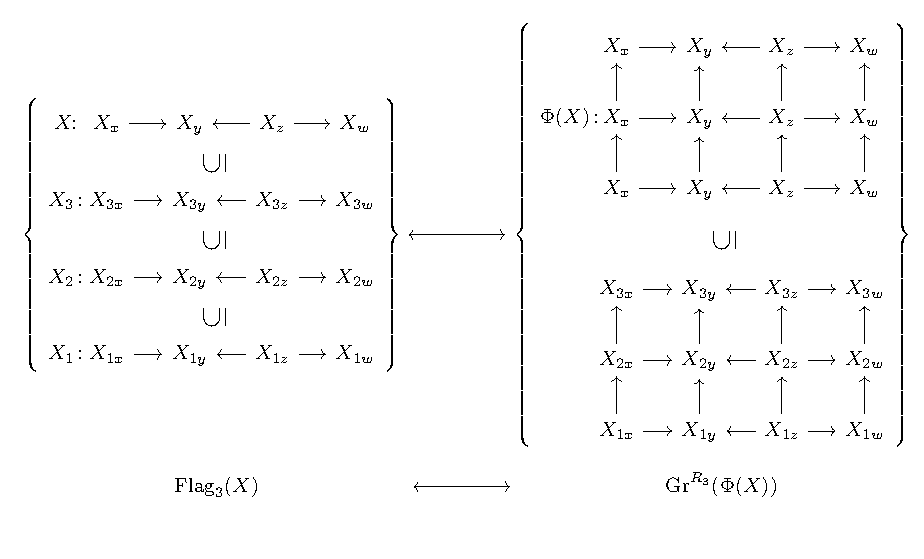
\includegraphics[width=0.9\linewidth]{figures/bigpic.pdf}
		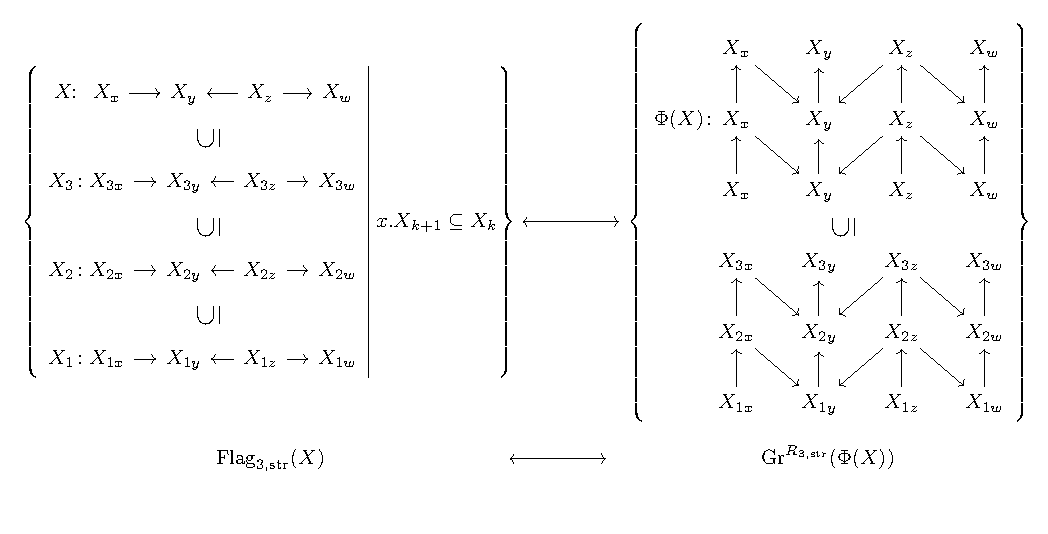
\includegraphics[width=\linewidth]{figures/bigpic2.pdf}
%		\captionsetup{labelformat=empty}
		\caption{}
		\label{fig:flagasgr}
	\end{figure}
\end{center}
\end{eg}
In many cases, the proof of the strict case and the non-strict case is the same, so we often treat them in the same way. For example, we may abbreviate the formula in Proposition \ref{prop:flag=gr} as 
$$\Flag{}(X)\cong \Gr(\Phi(X)).$$
\subsection{Dimension vector}In this subsection we recall some notations of dimension vectors.
\begin{defn}[Dimension vector]
For a quiver $Q$ and a representation $M \in \Rep(Q)$, the dimension vector of $Q$ is defined as the element in the set $\prod_{i \in v(Q)} \mathbb{Z}$, and the dimension vector of $M$ is defined as
$$\dimv M:=(\dim_K M_i)_{i \in v(Q)}.$$
Similarly, for a bounded quiver algebra $R=KQ/I$ and a module $T \in \Mod(R)$, the dimension vector of $R$ just means the dimension vector of $Q$, and the dimension vector of $T$ is defined as
$$\dimv T:=(\dim_K T_i)_{i \in v(Q)}.$$
\end{defn}
Now we can write (strict) partial flag and Grassmannian as disjoint union of several pieces. Take the nonstrict case as an example. Fix a dimension vector $\dimvec{f}$ of $R_d$, since $v(Q_d)=v(Q) \times \{1,\ldots,d\}$ it can be viewed as $d$ dimension vectors $(\dimvec{f_1},\ldots,\dimvec{f_d})$. Define
\begin{equation*}
\begin{aligned}
  \Flagd_{,\dimvec{f}}(X):=\;&\left\{ 0 \subseteq M_1 \subseteq \cdots M_d \subseteq X \;\middle|\; \dimv M_k=\dimvec{f_k} \right\}  \\ 
  \Gralg{R}_{\dimvec{f}}(T):=\;&\{T' \subseteq T \text{ with } \dimv T'=\dimvec{f}   \}
\end{aligned}
\end{equation*}
then from the Proposition \ref{prop:flag=gr} we get 
$$\Flagd_{,\dimvec{f}}(X) \cong \Gralg{R}_{\dimvec{f}}(\Phi(X)).$$

Finally, we need to define the ``Euler form" of two dimension vectors, for this we need to define the set of virtual arrows of quiver $Q_d$ and $Q_{d,str}$.
\begin{defn}[Virtual arrows of quiver $Q_d$]
For $d \geqslant 1$, the virtual arrows of quiver $Q_d$ is defined as a triple $\big(va(Q_d),s,t\big)$, where
$$va(Q_d):=a(Q) \times \{1,\ldots, d-1 \}$$
is a finite set, and $s,t: va(Q_d) \longrightarrow v(Q_d)$ are maps defined by
$$s\big((i\rightarrow j,r)\big)=(i,r) \qquad t \big((i\rightarrow j,r)\big)=(j,r+1).$$
\end{defn}
\begin{defn}[Virtual arrows of quiver $Q_{d,str}$]
For $d \geqslant 2$, the virtual arrows of quiver $Q_{d,str}$ is defined as a triple $\big(va(Q_{d,str}),s,t\big)$, where
$$va(Q_{d,str}):=a(Q) \times \{2,\ldots, d-1 \}$$
is a finite set, and $s,t: va(Q_{d,str}) \longrightarrow v(Q_{d,str})$ are maps defined by
$$s\big((i\rightarrow j,r)\big)=(i,r) \qquad t \big((i\rightarrow j,r)\big)=(j,r).$$
\end{defn}
\begin{center}
	\begin{figure}[ht]
		\vspace{0cm}
		\centering
% https://q.uiver.app/?q=WzAsMzEsWzAsMiwiXFxidWxsZXQiXSxbMiwyLCJcXGJ1bGxldCJdLFs0LDIsIlxcYnVsbGV0Il0sWzYsMiwiXFxidWxsZXQiXSxbNywyLCJcXGJ1bGxldCJdLFs5LDIsIlxcYnVsbGV0Il0sWzExLDIsIlxcYnVsbGV0Il0sWzEzLDIsIlxcYnVsbGV0Il0sWzcsMSwiXFxidWxsZXQiXSxbOSwxLCJcXGJ1bGxldCJdLFsxMSwxLCJcXGJ1bGxldCJdLFsxMywxLCJcXGJ1bGxldCJdLFs3LDAsIlxcYnVsbGV0Il0sWzksMCwiXFxidWxsZXQiXSxbMTEsMCwiXFxidWxsZXQiXSxbMTMsMCwiXFxidWxsZXQiXSxbMTQsMiwiXFxidWxsZXQiXSxbMTYsMiwiXFxidWxsZXQiXSxbMTQsMSwiXFxidWxsZXQiXSxbMTQsMCwiXFxidWxsZXQiXSxbMTYsMSwiXFxidWxsZXQiXSxbMTgsMSwiXFxidWxsZXQiXSxbMTgsMCwiXFxidWxsZXQiXSxbMjAsMSwiXFxidWxsZXQiXSxbMjAsMiwiXFxidWxsZXQiXSxbMjAsMCwiXFxidWxsZXQiXSxbMTgsMiwiXFxidWxsZXQiXSxbMTYsMCwiXFxidWxsZXQiXSxbMywzLCJcXGhzcGFjZXstMWNtfVFcXGhzcGFjZXstMWNtfSJdLFsxMCwzLCJcXGhzcGFjZXstMWNtfVFfM1xcaHNwYWNley0xY219Il0sWzE3LDMsIlxcaHNwYWNley0xY219UV97MyxzdHJ9XFxoc3BhY2V7LTFjbX0iXSxbMCwxXSxbMiwxXSxbMiwzXSxbNCw1XSxbNiw1XSxbNiw3XSxbOCw5XSxbMTAsOV0sWzEwLDExXSxbMTIsMTNdLFsxNCwxM10sWzE0LDE1XSxbOCwxMl0sWzQsOF0sWzUsOV0sWzksMTNdLFsxMCwxNF0sWzYsMTBdLFs3LDExXSxbMTEsMTVdLFsxOCwxN10sWzE5LDIwXSxbMjEsMTddLFsyMiwyMF0sWzIyLDIzXSxbMjEsMjRdLFsyMywyNV0sWzI0LDIzXSxbMjYsMjFdLFsyMSwyMl0sWzE3LDIwXSxbMjAsMjddLFsxOCwxOV0sWzE2LDE4XSxbOCwxMywiIiwxLHsiY29sb3VyIjpbMCwxMDAsNjBdfV0sWzQsOSwiIiwxLHsiY29sb3VyIjpbMCwxMDAsNjBdfV0sWzEwLDEzLCIiLDEseyJjb2xvdXIiOlswLDEwMCw2MF19XSxbNiw5LCIiLDEseyJjb2xvdXIiOlswLDEwMCw2MF19XSxbNiwxMSwiIiwxLHsiY29sb3VyIjpbMCwxMDAsNjBdfV0sWzEwLDE1LCIiLDEseyJjb2xvdXIiOlswLDEwMCw2MF19XSxbMTgsMjAsIiIsMSx7ImNvbG91ciI6WzAsMTAwLDYwXX1dLFsyMSwyMCwiIiwxLHsiY29sb3VyIjpbMCwxMDAsNjBdfV0sWzIxLDIzLCIiLDEseyJjb2xvdXIiOlswLDEwMCw2MF19XV0=
\[\begin{tikzcd}[column sep=3mm, row sep=5mm]
	&&&&&&&[5mm] \bullet && \bullet && \bullet && \bullet &[5mm] \bullet && \bullet && \bullet && \bullet \\
	&&&&&&& \bullet && \bullet && \bullet && \bullet & \bullet && \bullet && \bullet && \bullet \\
	\bullet && \bullet && \bullet && \bullet & \bullet && \bullet && \bullet && \bullet & \bullet && \bullet && \bullet && \bullet \\[-5mm]
	&&& {\hspace{-1cm}Q\hspace{-1cm}} &&&&&&& {\hspace{-1cm}Q_3\hspace{-1cm}} &&&&&&& {\hspace{-1cm}Q_{3,str}\hspace{-1cm}}
	\arrow[from=3-1, to=3-3]
	\arrow[from=3-5, to=3-3]
	\arrow[from=3-5, to=3-7]
	\arrow[from=3-8, to=3-10]
	\arrow[from=3-12, to=3-10]
	\arrow[from=3-12, to=3-14]
	\arrow[from=2-8, to=2-10]
	\arrow[from=2-12, to=2-10]
	\arrow[from=2-12, to=2-14]
	\arrow[from=1-8, to=1-10]
	\arrow[from=1-12, to=1-10]
	\arrow[from=1-12, to=1-14]
	\arrow[from=2-8, to=1-8]
	\arrow[from=3-8, to=2-8]
	\arrow[from=3-10, to=2-10]
	\arrow[from=2-10, to=1-10]
	\arrow[from=2-12, to=1-12]
	\arrow[from=3-12, to=2-12]
	\arrow[from=3-14, to=2-14]
	\arrow[from=2-14, to=1-14]
	\arrow[from=2-15, to=3-17]
	\arrow[from=1-15, to=2-17]
	\arrow[from=2-19, to=3-17]
	\arrow[from=1-19, to=2-17]
	\arrow[from=1-19, to=2-21]
	\arrow[from=2-19, to=3-21]
	\arrow[from=2-21, to=1-21]
	\arrow[from=3-21, to=2-21]
	\arrow[from=3-19, to=2-19]
	\arrow[from=2-19, to=1-19]
	\arrow[from=3-17, to=2-17]
	\arrow[from=2-17, to=1-17]
	\arrow[from=2-15, to=1-15]
	\arrow[from=3-15, to=2-15]
	\arrow[color={rgb,255:red,255;green,51;blue,51}, from=2-8, to=1-10]
	\arrow[color={rgb,255:red,255;green,51;blue,51}, from=3-8, to=2-10]
	\arrow[color={rgb,255:red,255;green,51;blue,51}, from=2-12, to=1-10]
	\arrow[color={rgb,255:red,255;green,51;blue,51}, from=3-12, to=2-10]
	\arrow[color={rgb,255:red,255;green,51;blue,51}, from=3-12, to=2-14]
	\arrow[color={rgb,255:red,255;green,51;blue,51}, from=2-12, to=1-14]
	\arrow[color={rgb,255:red,255;green,51;blue,51}, from=2-15, to=2-17]
	\arrow[color={rgb,255:red,255;green,51;blue,51}, from=2-19, to=2-17]
	\arrow[color={rgb,255:red,255;green,51;blue,51}, from=2-19, to=2-21]
\end{tikzcd}\]
		\caption{virtual arrow(red): can be thought as the ``face" of the quiver}
		\label{fig:virtualarrow}
	\end{figure}
\end{center}
\begin{defn}[Euler form of $R$]
Let $R$ be a bounded quiver algebra defined in Definition \ref{def:bqa} or \ref{def:bqastr}. We denote
\begin{equation*}
\begin{aligned}
	v(R):&= \{\text{vertices in quiver $Q_d$ or $Q_{d,str}$}\} \\
	a(R):&= \{\text{arrows in quiver $Q_d$ or $KQ_{d,str}$}\} \\
	va(R):&= \{\text{virtual arrows in quiver $Q_d$ or $Q_{d,str}$}\} \\
\end{aligned}
\end{equation*}

For two dimension vectors $\dimvec{f},\dimvec{g}$ of $R$, the Euler form $\left< \dimvec{f},\dimvec{g}\right>_R$ is defined by
	$$\left< \dimvec{f},\dimvec{g}\right>_R:= \sum_{i \in v(R)} f_ig_i - \sum_{b \in a(R)} f_{s(b)}g_{t(b)}+ \sum_{c \in va(R)} f_{s(c)}g_{t(c)}$$
\end{defn}
\subsection{Ext-vanishing properties}
We would like to show some higher rank extension group to be 0, which would be a key ingredient in the proof of the next section.

For a bounded quiver algebra $R$ defined in Definition \ref{def:bqa} or \ref{def:bqastr}, we have a standard resolution for every $R$-module $T$: 
% https://q.uiver.app/?q=WzAsMTIsWzAsMCwiMCJdLFsxLDAsIlxcYmlnb3BsdXNfe1xcc3Vic3RhY2t7YyBcXGluIHZhKFEpXFxcXGM9Yl8xY18xPWJfMmNfMn19IFJlX3t0KGMpfSBcXG90aW1lc19LIGVfe3MoYyl9VCJdLFsyLDAsIlxcYmlnb3BsdXNfe2IgXFxpbiBhKFEpfSBSZV97dChiKX0gXFxvdGltZXNfSyBlX3tzKGIpfVQiXSxbMywwLCJcXGJpZ29wbHVzX3tpIFxcaW4gdihRKX0gUmVfe2l9IFxcb3RpbWVzX0sgZV97aX1UIl0sWzQsMCwiVCJdLFs1LDAsIjAiXSxbMSwxLCJyIFxcb3RpbWVzIHgiXSxbMiwxLCJcXHN1YnN0YWNre1xccGhhbnRvbXsrfXJjXzEgXFxvdGltZXMgeCArciBcXG90aW1lcyBiXzF4XFxcXC1yY18yIFxcb3RpbWVzIHggLXIgXFxvdGltZXMgYl8yeH0iXSxbMywxLCJyIFxcb3RpbWVzIHgiXSxbNCwxLCJyeCJdLFsyLDIsInIgXFxvdGltZXMgeCJdLFszLDIsInJiIFxcb3RpbWVzIHgtciBcXG90aW1lcyBieCJdLFswLDFdLFsxLDJdLFsyLDNdLFszLDRdLFs0LDVdLFs2LDcsIiIsMCx7InN0eWxlIjp7InRhaWwiOnsibmFtZSI6Im1hcHMgdG8ifX19XSxbOCw5LCIiLDAseyJzdHlsZSI6eyJ0YWlsIjp7Im5hbWUiOiJtYXBzIHRvIn19fV0sWzEwLDExLCIiLDAseyJzdHlsZSI6eyJ0YWlsIjp7Im5hbWUiOiJtYXBzIHRvIn19fV1d
\[
\begin{tikzcd}[row sep=0mm,column sep=3mm]
	0 & {\displaystyle\bigoplus_{\substack{c \in va(Q)\\c=b_1c_1=b_2c_2}} \hspace{-5mm}Re_{t(c)} \otimes_K e_{s(c)}T} & {\displaystyle\bigoplus_{b \in a(Q)}\hspace{-2mm} Re_{t(b)} \otimes_K e_{s(b)}T} & {\displaystyle\bigoplus_{i \in v(Q)}\hspace{-2mm} Re_{i} \otimes_K e_{i}T} & T & 0 \\
	& {\hspace{10mm} r \otimes x} & {\substack{\phantom{+}rc_1 \otimes x +r \otimes b_1x\\-rc_2 \otimes x -r \otimes b_2x}\hspace{-5mm}} & {\hspace{6mm}r \otimes x} & rx \\
	&& {\hspace{6mm}r \otimes x} & {rb \otimes x-r \otimes bx\hspace{-3mm}}
	\arrow[from=1-1, to=1-2]
	\arrow[from=1-2, to=1-3]
	\arrow[from=1-3, to=1-4]
	\arrow[from=1-4, to=1-5]
	\arrow[from=1-5, to=1-6]
	\arrow[maps to, from=2-2, to=2-3]
	\arrow[maps to, from=2-4, to=2-5]
	\arrow[maps to, from=3-3, to=3-4]
\end{tikzcd}
\]
\begin{lemma}\label{lm:Extvan}
Let $M,N,X,S \in \Rep(Q)$, $V,W,T \in \Mod(R)$.
\begin{enumerate}[(1)]
	\item $\gldim R \leqslant 2$;\label{lm:gldim}
	\item The functor $\Phi:\Rep(Q) \longrightarrow \Mod(R)$ is exact and fully faithful;\label{lm:functorisexact}
	\item $\Phi$ maps projective module to projective module, and maps injective module to injective module;\label{lm:toproj}
	\item $\Ext^i_{KQ}(M,N) \cong \Ext^i_{R}(\Phi(M),\Phi(N))$;\label{lm:isoofext}
	\item $\projdim \Phi(M) \leqslant 1, \injdim \Phi(M) \leqslant 1$;\label{lm:projdim}
\end{enumerate}
\end{lemma}
\begin{proof}$\,$

For (\ref{lm:gldim}), this follows from the standard resolution.

For (\ref{lm:functorisexact}), it's clear. You can also follow \cite[Lemma 2.3]{maksimau2019flag}.
%if we have the short exact sequence in $\Rep(Q)$:
%$$0\longrightarrow X \longrightarrow Y \longrightarrow S \longrightarrow 0$$
%then for each vector $i\in v(Q)$, we have the short exact sequence 
%$$0\longrightarrow X_i \longrightarrow Y_i \longrightarrow S_i \longrightarrow 0,$$
%which is equivalent to the short exact sequence 
%$$0\longrightarrow \Phi(X)_{(i,r)} \longrightarrow \Phi(Y)_{(i,r)} \longrightarrow \Phi(S)_{(i,r)} \longrightarrow 0,$$
%for every vector $(i,r)$ in the extended quiver, so the complex
%$$0\longrightarrow \Phi(X) \longrightarrow \Phi(Y) \longrightarrow \Phi(S) \longrightarrow 0$$
%is exact.

For (\ref{lm:toproj}), we reduced to the case of indecomposable projective modules, and observe that $$\Phi(P(i))=P\big((i,1)\big),\qquad\Phi(I(i))=I\big((i,d)\big).$$

For (\ref{lm:isoofext}), it comes from the fact that $\Phi$ is fully faithful and maps projective module to projective module.
%the isomorphism 
%$$\Ext^i_{KQ}(M,N) \cong \Ext^i_{R}(\Phi(M),\Phi(N))$$
%follows by the projective resolution of $M$.
%the surjection of map
%$$\Hom_{KQ}(M,N) \longrightarrow \Hom_{R}(\Phi(M),\Phi(N))$$
%follows by the commutative diagram:
%
%\begin{center}
%% https://tikzcd.yichuanshen.de/#N4Igdg9gJgpgziAXAbVABwnAlgFyxMJZABgBpiBdUkANwEMAbAVxiRAFkB9LEAX1PSZc+QijIBGKrUYs2XHv0HY8BIuPJT6zVohAA5bnwEgMykWtKTqW2boMKpMKAHN4RUADMAThAC2SdRAcCCQAZmsZHRAAHWi0AAssTmAACixSLwBKXiNPH39EQOCkMmltNliASShckG8-MOpixAAmCPLdKprFOvySppDW9tsYuMTktIyAanFsvgpeIA
%\begin{tikzcd}
%M_i \arrow[r, "{\phi_{(i,r+1)}}"]                & N_i                  \\
%M_i \arrow[r, "{\phi_{(i,r)}}"] \arrow[u, "\Id"] & N_i \arrow[u, "\Id"]
%\end{tikzcd}
%\end{center}

For (\ref{lm:projdim}), Notice that the minimal projective resolution of $M$ is of length 1, and $\Phi(-)$ sends projective resolution of $M$ to projective resolution of $\Phi(M)$ by  (\ref{lm:toproj}), thus we get $\projdim \Phi(M) \leqslant 1$. The injective dimension of $\Phi(M)$ is computed in the similar way.
\end{proof}
Moreover, we will have the key lemma which will be crucial in the later use.
\begin{lemma}\label{lm:Ext2van}
Let $X,S \in \Rep(Q)$ be any representation. Suppose $V \subseteq \Phi(X), W \subseteq \Phi(S)$, then $\Ext^2_{R}(W,T)=0, \Ext^2_{R}(T,\Phi(X)/V)=0$.
\end{lemma}
\begin{proof}
The short exact sequence 
$$0 \longrightarrow W \longrightarrow \Phi(S) \longrightarrow \Phi(S)/W \longrightarrow 0$$
induces the long exact sequence 
$$\cdots \longrightarrow \Ext^2_{R}(\Phi(S),T) \longrightarrow \Ext^2_{R}(W,T) \longrightarrow \Ext^3_{R}(\Phi(S)/W,T) \longrightarrow \cdots$$
By Lemma \ref{lm:Extvan} (\ref{lm:gldim}) and (\ref{lm:projdim}), $\Ext^3_{R}(\Phi(S)/W,T)$ and $\Ext^2_{R}(\Phi(S),T)$ are both $0$, so $\Ext^2_{R}(W,T)=0$.

Similarly, from the short exact sequence
$$0 \longrightarrow V \longrightarrow \Phi(X) \longrightarrow \Phi(X)/V \longrightarrow 0$$
we get the induced long exact sequence
$$\cdots \longrightarrow \Ext^2_{R}(T,\Phi(X)) \longrightarrow \Ext^2_{R}(T,\Phi(X)/V) \longrightarrow \Ext^3_{R}(T,V) \longrightarrow \cdots$$
so $\Ext^2_{R}(T,\Phi(X)/V)=0$.
\end{proof}
We will frequently use extension groups as well as long exact sequences, so now it's time to shorten some notations. For the $Q$-representations $M,N$ and $R$-modules $T,T'$, we denote  
\begin{equation*}
\begin{aligned}[]
	[M,N]^i:&=\dim_K \Ext^i_{KQ} (M,N),\qquad [M,N]:=\dim_K \Hom_{KQ} (M,N)\\
	[T,T']^i:&=\dim_K \Ext^i_R (T,T'),\qquad\hspace{0.5cm} [T,T']:=\dim_K \Hom_R (T,T')
\end{aligned}
\end{equation*}
and write the Euler form as
$$\left< T,T'\right>_R:= \sum_{i=0}^{\infty} (-1)^i [T,T']^i \quad=[T,T']-[T,T']^1+[T,T']^2.$$
\begin{corollary}
	For two $R$-modules $T,T'$, we have
	$$	\left< T,T'\right>_R = 	\left< \dimv T,\dimv T'\right>_R.$$
\end{corollary}
\begin{proof}
Just compute $\left< T,T'\right>_R$ by applying the functor $\Hom_R(-,T')$ to the standard resolution of $R$-module $T$.
\end{proof}
\subsection{How much do we understand the quiver representation?}
To understand the category $\Rep(Q)$, one should understand indecomposable modules(as well as their relations). This has almost been done in the Auslander-Reiten theory. For example, when the quiver $Q$ is of Dynkin type, then there are only finite indecomposable representations(up to isomorphism) and each indecomposable representation corresponds to the positive root of Dynkin diagram. One can compute the Auslander-Reiten quiver by knitting algorithm and get the structure of indecomposable representations. Moreover, one can directly get Hom space between $M$ and $N$ by looking at nontrivial paths from $M$ to $N$\footnote{These paths may be linear dependent, so it's not too easy.}.

We will use the Auslander-Reiten quiver to find ``good monomorphisms" in Section \ref{sec:Dynkin},\ref{sec:affine}. For more informations about Auslander-Reiten theory, one can see \cite{crawley1992lectures}.
%%%%%%%%%%%%%%%%%%%%%%%%%%%%%%%%%%%%%%%%%%%%%%%%%%%%%%%%%%%%%%%%%%%%%%%%%%%%%%%%%%%%%%%%%%%%%

\section{Main Theorem}\label{sec:mainthm}
In this section we state and prove the main theorems, which would be essentially used in the Section \ref{sec:Dynkin} and \ref{sec:affine}.
   
Let $\eta: 0\longrightarrow X \stackrel{\iota}{\longrightarrow} Y \stackrel{\pi}{\longrightarrow} S \longrightarrow 0$ be a short exact sequence in $Rep(Q)$. Consider the canonical \textbf{non-continuous} map
$$\Psi: \Grr(\Phi(Y)) \longrightarrow \Grr(\Phi(X)) \times \Grr(\Phi(S)) \qquad U \longmapsto \left([\Phi(\iota)]^{-1}(U),[\Phi(\pi)](U)   \right)$$
and  $\Psi_{\dimvec{f},\dimvec{g}}$ is the map $\Psi$ restricted to the preimage of $\Grr_{\dimvec{f}}(\Phi(X)) \times \Grr_{\dimvec{g}}(\Phi(S))$.

%The goal of this section is to prove the following theorems:
\begin{theorem}\label{thm:main1}
	When $\eta$ splits, $\Psi$ is surjective. Moreover, $\Psi_{\dimvec{f},\dimvec{g}}$ is a Zarisky-locally trivial affine bundle of rank $\left< \dimvec{g},\dimv \Phi(X) - \dimvec{f}\right>_R$.
\end{theorem}
\begin{theorem}[follows {\cite[Theorem 32]{irelli2019cell}}]\label{thm:main2}
	When $\eta$ does not split and $[S,X]^1=1$, 
	$$\Img \Psi_{\dimvec{f},\dimvec{g}} = \bigg(\Grr_{\dimvec{f}}(\Phi(X)) \times \Grr_{\dimvec{g}}(\Phi(S)) \bigg) \setminus \bigg(\Grr_{\dimvec{f}}(\Phi(X_S)) \times \Grr_{\dimvec{g}-\dimv \Phi(S^X)}\left(\Phi(S/S^X)\right) \bigg)$$
	where 
	\begin{equation*}
	\begin{aligned}
	X_S:&= \max \left\{ M \subseteq X \,\middle|\; [S,X/M ]^1=1 \right\} \subseteq X\\
	S^X:&= \max \left\{ M \subseteq S \,\middle|\; [M,X]^1=1 \right\} \subseteq S
	\end{aligned}
	\end{equation*}
Moreover, $\Psi_{\dimvec{f},\dimvec{g}}$ is a Zarisky-locally trivial affine bundle of rank $\left< \dimvec{g},\dimv \Phi(X) - \dimvec{f}\right>_R$ over $\Img \Psi_{\dimvec{f},\dimvec{g}}$.
\end{theorem}

We will spend the rest of the section proving these theorems. We investigate the image as well as the fiber of $\Psi$ respectively.
\begin{lemma}[follows {\cite[Lemma 21]{irelli2019cell}}]\label{lm:split}
The element $(V,W) \in \Grr(\Phi(X)) \times \Grr(\Phi(S))$ lies in the image of $\Psi$ if and only if the canonical map $\Ext^1(\Phi(S),\Phi(X)) \longrightarrow \Ext^1(W,\Phi(X)/V)$ maps $\eta$ to 0.
\end{lemma}
\begin{proof}
	The canonical map is defined as follows:
% https://q.uiver.app/?q=WzAsMjIsWzQsMCwiXFxQaGkoWCkiXSxbNCwxLCJcXFBoaShYKSJdLFs0LDIsIlxcUGhpKFgpL1YiXSxbNSwxLCJcXHBpXnstMX0oVykiXSxbNSwwLCJcXFBoaShZKSJdLFs1LDIsIlxccGleey0xfShXKS9WIl0sWzYsMSwiVyJdLFs2LDIsIlciXSxbNiwwLCJcXFBoaShTKSJdLFszLDAsIjAiXSxbNywwLCIwIl0sWzMsMSwiMCJdLFs3LDEsIjAiXSxbMywyLCIwIl0sWzcsMiwiMCJdLFsyLDAsIlxcRXh0XjEoXFxQaGkoUyksXFxQaGkoWCkpIl0sWzIsMSwiXFxFeHReMShXLFxcUGhpKFgpKSJdLFsyLDIsIlxcRXh0XjEoVyxcXFBoaShYKS9WKSJdLFswLDAsIlxcZXRhIl0sWzAsMiwiXFxiYXJ7XFxldGF9Il0sWzEsMCwiXFxpbiJdLFsxLDIsIlxcaW4iXSxbMSwyXSxbMSwwLCIiLDIseyJsZXZlbCI6Miwic3R5bGUiOnsiaGVhZCI6eyJuYW1lIjoibm9uZSJ9fX1dLFszLDRdLFszLDVdLFs2LDcsIiIsMCx7ImxldmVsIjoyLCJzdHlsZSI6eyJoZWFkIjp7Im5hbWUiOiJub25lIn19fV0sWzYsOF0sWzksMF0sWzAsNF0sWzQsOCwiXFxwaSJdLFs4LDEwXSxbMTEsMV0sWzEsM10sWzMsNl0sWzYsMTJdLFsxMywyXSxbMiw1XSxbNSw3XSxbNywxNF0sWzE1LDE2XSxbMTYsMTddLFsxOCwxOSwiIiwwLHsic3R5bGUiOnsidGFpbCI6eyJuYW1lIjoibWFwcyB0byJ9fX1dXQ==
\[\begin{tikzcd}
	\eta &[-30pt] \in &[-30pt] {\Ext^1(\Phi(S),\Phi(X))} & 0 & {\Phi(X)} & {\Phi(Y)} & {\Phi(S)} & 0 \\
	&& {\Ext^1(W,\Phi(X))} & 0 & {\Phi(X)} & {\pi^{-1}(W)} & W & 0 \\
	{\bar{\eta}} & \in & {\Ext^1(W,\Phi(X)/V)} & 0 & {\Phi(X)/V} & {\pi^{-1}(W)/V} & W & 0
	\arrow[from=2-5, to=3-5]
	\arrow[Rightarrow, no head, from=2-5, to=1-5]
	\arrow[from=2-6, to=1-6]
	\arrow[from=2-6, to=3-6]
	\arrow[Rightarrow, no head, from=2-7, to=3-7]
	\arrow[from=2-7, to=1-7]
	\arrow[from=1-4, to=1-5]
	\arrow[from=1-5, to=1-6]
	\arrow["\pi", from=1-6, to=1-7]
	\arrow[from=1-7, to=1-8]
	\arrow[from=2-4, to=2-5]
	\arrow[from=2-5, to=2-6]
	\arrow[from=2-6, to=2-7]
	\arrow[from=2-7, to=2-8]
	\arrow[from=3-4, to=3-5]
	\arrow[from=3-5, to=3-6]
	\arrow[from=3-6, to=3-7]
	\arrow[from=3-7, to=3-8]
	\arrow[from=1-3, to=2-3]
	\arrow[from=2-3, to=3-3]
	\arrow[maps to, from=1-1, to=3-1]
\end{tikzcd}\]
so $\bar{\eta}=0$ if and only if the last short exact sequence splits, that means, there exist a submodule $U \subseteq \Phi(Y)$, such that $\pi(U)=W$ and $U \cap \Phi(X) =V$.

\end{proof}

\begin{corollary}\label{cor:img1}
	Resume the notations of Lemma \ref{lm:split} When $\eta$ splits, then $\Psi$ is surjective.
\end{corollary}
\begin{lemma}
	the canonical map $\Ext^1(\Phi(S),\Phi(X)) \longrightarrow \Ext^1(W,\Phi(X)/V)$ is surjective.
\end{lemma}
\begin{proof}
	By using the long exact sequence of Extension groups and the Lemma \ref{lm:Ext2van}, the maps
	$$\Ext^1(\Phi(S),\Phi(X)) \longrightarrow \Ext^1(W,\Phi(X))\qquad \Ext^1(W,\Phi(X)) \longrightarrow \Ext^1(W,\Phi(X)/V)$$
	are both surjective. Thus the composition is also surjective.
\end{proof}
\begin{corollary}[]\label{cor:0or1}
	Let $W \subseteq \Phi(S), V \subseteq \Phi(X)$ be $R$-submodules, then
	$$[W,\Phi(X)/V]^1 \leqslant [\Phi(S),\Phi(X)]^1=[S,X]^1,$$
	In particular, when $[S,X]^1=1$, we get $[W,\Phi(X)/V]^1=0 \text{ or }1$.
	
	Suppose $\eta$ generates $\Ext^1(S,X)$, then 
	$$(V,W) \in \Img \Psi \iff [W,\Phi(X)/V]^1=0.$$
\end{corollary}

In the case where $\eta$ generates $\Ext^1(S,X)$, we want to describe $\Img \Psi$ more precisely. For this reason we need to introduce two new $R$-modules:
	\begin{equation*}
	\begin{aligned}
	\widetilde{X_S}:&= \max \left\{ V \subseteq \Phi(X) \,\middle|\; [\Phi(S),\Phi(X)/V ]^1=1 \right\} \subseteq \Phi(X)\\
	\widetilde{S^X}:&= \max \left\{ W \subseteq \Phi(S) \,\middle|\; [W,\Phi(X)]^1=1 \right\} \subseteq \Phi(S)
	\end{aligned}
	\end{equation*}
$\widetilde{X_S}$ and $\widetilde{S^X}$ are well-defined because of the following lemma:
\begin{lemma}[follows {\cite[Lemma 27]{irelli2019cell}}]

\begin{enumerate}[(i)]
	\item[] 
	\item Let $V,V' \subset \Phi(X)$ such that $[\Phi(S),\Phi(X)/V ]^1=[\Phi(S),\Phi(X)/V']^1=1 .$ Then $[\Phi(S),\Phi(X)/V+V' ]^1=1$.
	\item  Let $W,W' \subset \Phi(S)$ such that $[W,\Phi(X)]^1=[W',\Phi(X)]^1=1 .$ Then $[W\cap W',\Phi(X)]^1=1$.
\end{enumerate}
\end{lemma}
\begin{proof}
We only prove (i). (ii) is similar.

From the short exact sequence 
$$0 \longrightarrow \Phi(X)/V\cap V' \longrightarrow \Phi(X)/V \oplus \Phi(X)/V' \longrightarrow \Phi(X)/V+V' \longrightarrow 0,$$
we get the long exact sequence
$$\hspace{-0.4cm}\cdots\rightarrow \Ext^1\!\!\left(\Phi(S),\textstyle\frac{\Phi(X)}{V\cap V'}\right) \rightarrow \Ext^1\!\!\left(\Phi(S),\textstyle\frac{\Phi(X)}{V}\right) \oplus \;\Ext^1\!\!\left(\Phi(S),\textstyle\frac{\Phi(X)}{V'}\right) \rightarrow \Ext^1\!\!\left(\Phi(S),\textstyle\frac{\Phi(X)}{V+ V'}\right) \rightarrow\cdots$$
By Corollary \ref{cor:0or1}, $[\Phi(S),\Phi(X)/V\cap V']^1\leqslant 1, \; [\Phi(S),\Phi(X)/V+V']^1\leqslant 1$, and this forces that $[\Phi(S),\Phi(X)/V+V']^1= 1$.
\end{proof}
\begin{lemma}[follows {\cite[Lemma 31(1)(2)]{irelli2019cell}}, and the proof is same]

Let $f:X \longrightarrow \tau S$ be a non-zero morphism, then $X_S=\ker (f)$; also, $\Phi(f): \Phi(X) \longrightarrow \Phi(\tau S)$ is a non-zero morphism, $\widetilde{X_S}=\ker (\Phi(f))$.
\end{lemma}
\begin{corollary}
	$\widetilde{X_S}=\Phi(X_S)$.\textcolor{black}{(since $\widetilde{X_S}=\ker (\Phi(f))=\Phi(\ker(f))=\Phi(X_S)$)}
\end{corollary}
By the similar argument, one can show that $\widetilde{S^X}=\Phi(S^X)$.
\begin{lemma}[follows {\cite[Lemma 31(6)]{irelli2019cell}}]
Given $V \subseteq \Phi(X)$ and $W \subseteq \Phi(S)$, we have 
$$[W,\Phi(X)/V]^1=0 \iff V \nsubseteq \Phi(X_S) \text{ or }W \nsupseteq \Phi(S^X).$$
\end{lemma}
\begin{proof}
$\Leftarrow$: without lose of generation suppose $V \nsubseteq \Phi(X_S)$, then
$$V \nsubseteq \Phi(X_S) \iff [\Phi(S),\Phi(X)/V ]^1=0 \Rightarrow  [W,\Phi(X)/V ]^1=0.$$

\hspace{0.8cm}$\Rightarrow$: If not, then $V \subseteq \Phi(X_S) \text{ and }W \supseteq \Phi(S^X)$, and\footnote{$[S^X,X/X_S]^1=1$ follows from \cite[Lemma 31(5)]{irelli2019cell}} 
$$[W,\Phi(X)/V]^1 \geqslant [\Phi(S^X),\Phi(X)/\Phi(X_S)]^1 =[S^X,X/X_S]^1=1.$$
We get the contradiction!
\end{proof}
\begin{corollary}\label{cor:img2}
When $\eta$ generates $\Ext^1(S,X)$, we have 
	$$\Img \Psi_{\dimvec{f},\dimvec{g}} = \bigg(\Grr_{\dimvec{f}}(\Phi(X)) \times \Grr_{\dimvec{g}}(\Phi(S)) \bigg) \setminus \bigg(\Grr_{\dimvec{f}}(\Phi(X_S)) \times \Grr_{\dimvec{g}-\dimv \Phi(S^X)}\left(\Phi(S/S^X)\right) \bigg)$$
\end{corollary}

\begin{lemma}
	For $(V,W) \in \Img \Psi$, the preimage of $(V,W)$ is a torsor of $\,\Hom_{R}(W,\Phi(X)/V)$. Or we could say, there is one non-canonical isomorphism
	$$\Psi^{-1}((V,W)) \cong \Hom_{R}(W,\Phi(X)/V).$$
\end{lemma}
\begin{proof}Recall the commutative diagram
% https://q.uiver.app/?q=WzAsMjIsWzQsMCwiXFxQaGkoWCkiXSxbNCwxLCJcXFBoaShYKSJdLFs0LDIsIlxcUGhpKFgpL1YiXSxbNSwxLCJcXHBpXnstMX0oVykiXSxbNSwwLCJcXFBoaShZKSJdLFs1LDIsIlxccGleey0xfShXKS9WIl0sWzYsMSwiVyJdLFs2LDIsIlciXSxbNiwwLCJcXFBoaShTKSJdLFszLDAsIjAiXSxbNywwLCIwIl0sWzMsMSwiMCJdLFs3LDEsIjAiXSxbMywyLCIwIl0sWzcsMiwiMCJdLFsyLDAsIlxcRXh0XjEoXFxQaGkoUyksXFxQaGkoWCkpIl0sWzIsMSwiXFxFeHReMShXLFxcUGhpKFgpKSJdLFsyLDIsIlxcRXh0XjEoVyxcXFBoaShYKS9WKSJdLFswLDAsIlxcZXRhIl0sWzAsMiwiXFxiYXJ7XFxldGF9Il0sWzEsMCwiXFxpbiJdLFsxLDIsIlxcaW4iXSxbMSwyXSxbMSwwLCIiLDIseyJsZXZlbCI6Miwic3R5bGUiOnsiaGVhZCI6eyJuYW1lIjoibm9uZSJ9fX1dLFszLDRdLFszLDVdLFs2LDcsIiIsMCx7ImxldmVsIjoyLCJzdHlsZSI6eyJoZWFkIjp7Im5hbWUiOiJub25lIn19fV0sWzYsOF0sWzksMF0sWzAsNF0sWzQsOCwiXFxwaSJdLFs4LDEwXSxbMTEsMV0sWzEsM10sWzMsNl0sWzYsMTJdLFsxMywyXSxbMiw1LCJcXGlvdGEiXSxbNSw3LCJcXHBpJyJdLFs3LDE0XSxbMTUsMTZdLFsxNiwxN10sWzE4LDE5LCIiLDAseyJzdHlsZSI6eyJ0YWlsIjp7Im5hbWUiOiJtYXBzIHRvIn19fV0sWzcsNSwiXFx0aGV0YSIsMix7ImN1cnZlIjotMywiY29sb3VyIjpbMzU4LDEwMCw2MF19LFszNTgsMTAwLDYwLDFdXV0=
\[\begin{tikzcd}
	\eta &[-30pt] \in & [-30pt]{\Ext^1(\Phi(S),\Phi(X))} & 0 & {\Phi(X)} & {\Phi(Y)} & {\Phi(S)} & 0 \\
	&& {\Ext^1(W,\Phi(X))} & 0 & {\Phi(X)} & {\pi^{-1}(W)} & W & 0 \\
	{\bar{\eta}} & \in & {\Ext^1(W,\Phi(X)/V)} & 0 & {\Phi(X)/V} & {\pi^{-1}(W)/V} & W & 0
	\arrow[from=2-5, to=3-5]
	\arrow[Rightarrow, no head, from=2-5, to=1-5]
	\arrow[from=2-6, to=1-6]
	\arrow[from=2-6, to=3-6]
	\arrow[Rightarrow, no head, from=2-7, to=3-7]
	\arrow[from=2-7, to=1-7]
	\arrow[from=1-4, to=1-5]
	\arrow[from=1-5, to=1-6]
	\arrow["\pi", from=1-6, to=1-7]
	\arrow[from=1-7, to=1-8]
	\arrow[from=2-4, to=2-5]
	\arrow[from=2-5, to=2-6]
	\arrow[from=2-6, to=2-7]
	\arrow[from=2-7, to=2-8]
	\arrow[from=3-4, to=3-5]
	\arrow["\iota", from=3-5, to=3-6]
	\arrow["{\pi'}", from=3-6, to=3-7]
	\arrow[from=3-7, to=3-8]
	\arrow[from=1-3, to=2-3]
	\arrow[from=2-3, to=3-3]
	\arrow[maps to, from=1-1, to=3-1]
	\arrow["\theta"', color={rgb,255:red,255;green,51;blue,58}, curve={height=-18pt}, from=3-7, to=3-6]
\end{tikzcd}\]
When $(V,W) \in \Img \Psi$, $\bar{\eta}$ is split, and each split morphism $\theta$ give us an element in $\Psi^{-1}((V,W))$. If we fix one split morphism $\theta_0$, then the other split morphisms are all of the form $\theta_0 + \textcolor{black}{\iota \circ} f$ where $f \in \Hom_{R}(W,\Phi(X)/V)$(and this form is unique). So
$$\Psi^{-1}((V,W)) \cong \{ \theta: \text{ split morphism} \} \cong \Hom_{R}(W,\Phi(X)/V).$$
\end{proof}
\begin{proof}[{Proof of Theorem \ref{thm:main1} and \ref{thm:main2}}]
We have already computed $\Img \Psi$ in Corollary \ref{cor:img1} and \ref{cor:img2}. For the rank of the affine bundle, we have 
\begin{equation*}
\begin{aligned}
(V,W) \in \Img \Psi_{\dimvec{f},\dimvec{g}} &\Longrightarrow [W,\Phi(X)/V]^1=0\\
& \Longrightarrow [W,\Phi(X)/V]=\left< W,\Phi(X)/V\right>_R=\left< \dimvec{f},\dimv \Phi(X)-\dimvec{g}\right>_R
\end{aligned}
\end{equation*}
\end{proof}
%%%%%%%%%%%%%%%%%%%%%%%%%%%%%%%%%%%%%%%%%%%%%%%%%%%%%%%%%%%%%%%%%%%%%%%%%%

\section{Application: Dynkin Case}\label{sec:Dynkin}
Before discussing the affine paving property, let me introduce some new numerical concepts, which can be seen as the measure of the ``complexity" of the representation.

Fix an \textbf{indecomposable} quiver representation $M \in \Rep(\mathbb{Q})$, we define the order of $M$ by
$$\ord(M):= \max_{i \in v(Q)} \dim_K M_i.$$
When the quiver $Q$ is of type $E$, we denote by $e \in v(Q)$ the unique vertex which is connected to three other vertices, and the number 
$$\orde(M):=\dim_K M_e=[P(e),M]$$
is equal to $\ord(M)$ unless $\orde(M)=0$.

By Theorem \ref{thm:main1}, we just need to focus on the case of indecomposable modules. The next lemma tells us, for the ``easy representation", we can prove the affine paving property easily.

\begin{lemma}[{follows \cite[Lemma 2.22]{maksimau2019flag}}]\label{lem:smallvecdim}
	For the representation $M \in \Rep(Q)$ satisfying $\ord(M) \leqslant 2$ and the dimension vector $\dimvec{f}$, the variety $\Grr_{\dimvec{f}}(\Phi(M))$ is either empty or is a singleton or is a direct product of some copies of $\mathbb{P}^1$.
\end{lemma}
\begin{proof}
	For each vertex $i$ of the bigger quiver, the dimension of $V_i$ is 0,1,2; then the variety $\Grr_{\dimvec{f}}(\Phi(M))$ is naturally included to a direct product of $\mathbb{P}^1$, and the information of arrows just reduce the number of $\mathbb{P}^1$(maybe to singleton or empty).
\end{proof}
\begin{corollary}[{\cite[Theorem 2.20]{maksimau2019flag}}]\label{cor:affinepavingofAD}
	Assume that $Q$ is a Dynkin quiver of type $A$ or $D$, $M \in \Rep(Q)$ is the representation. then the Grassmannian $\Grr(\Phi(M))$ has an affine paving.
\end{corollary}
\begin{corollary}\label{cor:affineADcase}
	Assume that $Q$ is a affine quiver of type $A$ or $D$, $M \in \Rep(Q)$ is the \textbf{regular quasi-simple} representation. then the Grassmannian $\Grr(\Phi(M))$ has an affine paving.
\end{corollary}
%We use rep 2 Cor 18.8.

\textbf{In the rest of this section we focus on the ``difficult" indecomposable representation of $E_6,E_7,E_8$.} The idea is to design the special route for each case, and use Theorem \ref{thm:main2} in the process. Notice that even though the Auslander-Reiten quivers look quite different for different quiver(with same type), they can have the same form is we use the number $\orde(M)$ to represent the representation $M$:\footnote{Some representations $M$ are hidden when $\orde(M)=0$. In \cite{bongartz1984critical} the Figure \ref{fig:startingfunction} is called the starting functions.}

\begin{center}
	\begin{figure}[ht]
		\vspace{0cm}
		\centering
		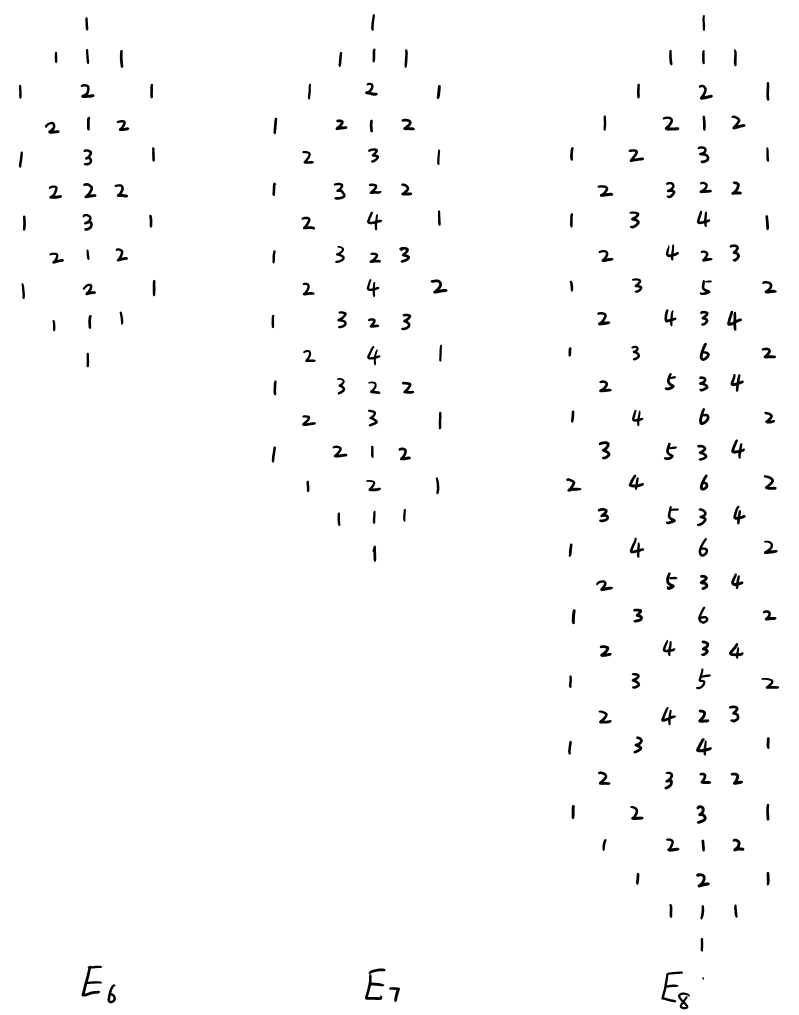
\includegraphics[width=6cm]{figures/startingfunction.png}
%		\captionsetup{labelformat=empty}
		\caption{central imformation of Auslander-Reiten quiver}
		\label{fig:startingfunction}
	\end{figure}
\end{center}

\begin{lemma}
	For every indecomposable representation $Y$ of type $E$ with $\ord(Y)>2$, there is a minimal section mono $f:X \longrightarrow Y$.
\end{lemma}
\begin{proof}
	Just observe the Auslander-Reiten sequence. The chosen minimal section monos are represented in Figure \ref{fig:minisecmono}. Notice that for the most time $\orde(-)$ is enough to guarantee the map to be a mono.
\end{proof}
	\begin{center}
		\begin{figure}[ht]
			\vspace{0cm}
			\centering
			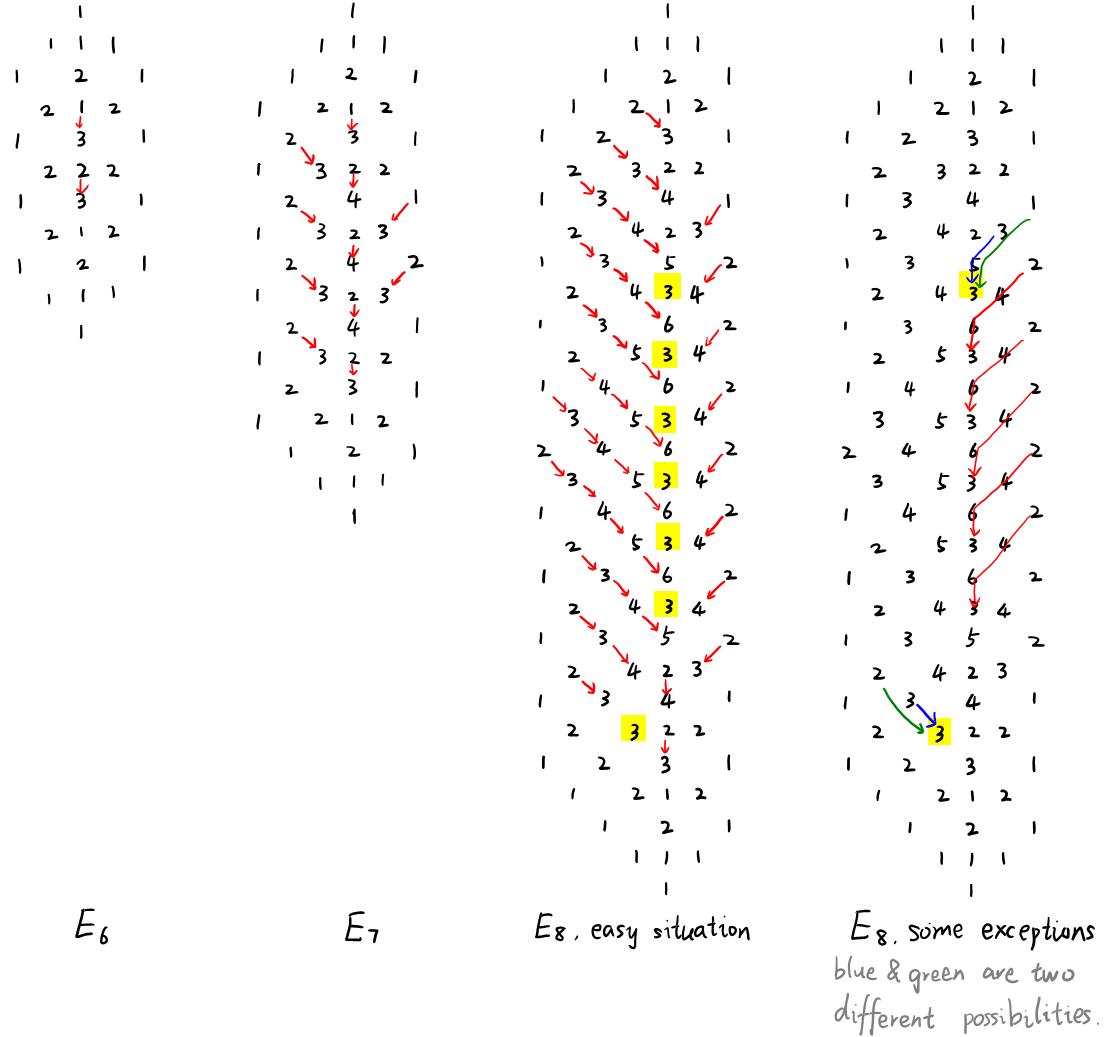
\includegraphics[width=7.5cm]{figures/minisecmono.png}
	%		\captionsetup{labelformat=empty}
			\caption{minimal section monos}
			\label{fig:minisecmono}
			\vspace{0.2cm}
		\end{figure}
	\end{center}
	
\begin{remark}
	The condition $\ord(Y)>2$ in the lemma can not be removed.
\end{remark}
\begin{lemma}\label{lem:value}
Let $X \hookrightarrow Y$ be an minimal section mono, and $S:=Y/X$ be the quotient. Then we have the short exact sequence 
$$\eta: 0 \longrightarrow X \longrightarrow Y \longrightarrow S \longrightarrow 0$$
and the following values:

\begin{center}
	\begin{figure}[ht]\label{fig:table}
		\vspace{0cm}
		\centering
		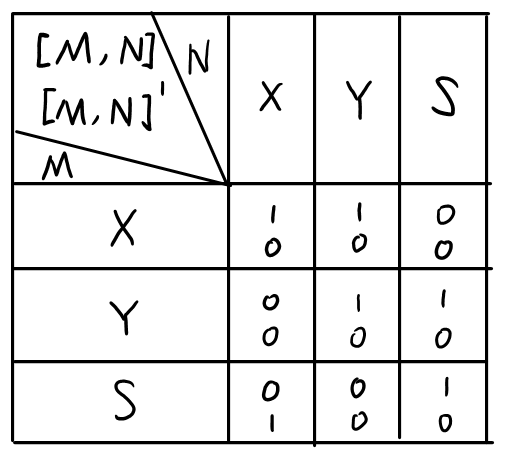
\includegraphics[width=5cm]{figures/table.png}
	\end{figure}
\end{center}

In particular, $S$ is indecomposable and rigid; $[S,X]^1 =1$, so $X_S$ and $S^X$ are well-defined.
\end{lemma}
\begin{proof}
We know that $[X,X]=[Y,Y]=1$ and $[X,X]^1=[Y,Y]^1=0$. By the definition of minimal section mono, we get
$[X,Y]=1, [Y,X]=0$ and $[X,Y]^1=[Y,X]^1=0$. By applying the functors $[Y,-],[-,S],[X,-],[-,X],[-Y]$ to the short exact sequence $\eta$ we get the results. 
\end{proof}
In the following two lemmas we will describe the representations $S^X$ and $X_S$ more clearly.
\begin{lemma} Take the same notations as in Lemma \ref{lem:value}. Then $S^X=S$.
\end{lemma}
\begin{proof}
	Let $\iota:N \longrightarrow S$ be a proper non-zero subrepresentation of $S$, we need to prove that $\iota^* \eta: 0\longrightarrow X \longrightarrow Y' \longrightarrow N \longrightarrow 0$ splits.
	

\begin{center}
\begin{tikzcd}
\iota^*\eta: & 0 \arrow[r] & X \arrow[r, hook'] \arrow[d, equal] & Y' \arrow[r] \arrow[d, "\eta", hook'] & N \arrow[r] \arrow[d, "\iota", hook'] & 0 \\
\eta:        & 0 \arrow[r] & X \arrow[r]                                       & Y \arrow[r]                           & S \arrow[r]                           & 0
\end{tikzcd}
\end{center}
	
	We decompose $Y'=\oplus_i Y_i'$ as the direct sum of indecomposable representations. Since the map $X\longrightarrow Y$ is the minimal section mono, we get $Y_i'=X$ or $Y_i'=Y$ or $X\stackrel{0}{\longrightarrow} Y_i'$ for all $i$.
	If there exists $i$ such that $Y_i'=X$, then $\iota^* $ splits; if there exists $i$ such that $Y_i'=Y$, then $\eta$ is isomorphism, we get $\iota$ is isomorphism; if for every $i$ the map $X \longrightarrow Y_i'$ is $0$, then the map $X \longrightarrow Y'$ is $0$, we also get the contradiction.
\end{proof}
\begin{lemma}[{follows \cite[Lemma 36]{irelli2019cell}, proof is exactly the same}]\label{lem:descriptionofX_S}
	Let $E \longrightarrow X$ be the minimal right almost split morphism ending in $X$, then we can decompose $E$ as $E=E' \oplus \tau X_1$. When $Y$ is not projective, $X_S$ is isomorphic to $\ker (E \longrightarrow \tau Y) \cong E' \oplus \ker (\tau X_1 \longrightarrow \tau Y)$; when $Y$ is projective, $X_S \cong E$.
\end{lemma}
\begin{corollary}
	When $X \longrightarrow Y$ is irreducible monomorphism, the representation $X_S$ is either $0$ or an indecomposable representation with property that $X_S \longrightarrow X$ is also an irreducible monomorphism.
\end{corollary}
\begin{remark}
	We can not copy everything in \cite[Lemma 56]{irelli2019cell}, sometimes it would happen that $X_S=F \oplus T$ with $F$ and $T$ indecomposable, $F \hookrightarrow X$ is irreducible but $T \longrightarrow X/F$ is not a good mono.
	
	For example, take the quiver of type $E_7$: 
	\begin{tikzcd}[row sep=3mm, column sep=5mm]
	                &                 &                 & \bullet \arrow[d] &                 &                 \\
	\bullet \arrow[r] & \bullet \arrow[r] & \bullet \arrow[r] & \bullet           & \bullet \arrow[l] & \bullet \arrow[l]
	\end{tikzcd}\\
	 take $Y=\representation{122321}{1}$, $X=\representation{112321}{1}$, then $X_S=\representation{111210}{1}\oplus \representation{000111}{0}=F \oplus T$, $X/F =\representation{001111}{0}$, the map $T \longrightarrow X/F$ is not a good mono.
	
	Luckily, we can avoid this bad situation by carefully choosing the minimal section mono $X \longrightarrow Y$. The minimal section monos I chose are presented in Figure \ref{fig:minisecmono}. In appendix we will write down the induction process in detail for some examples.
\end{remark}
%%%%%%%%%%%%%%%%%%%%%%%%%%%%%%%%%%%%%%%%%%%%%%%%%%%%%%%%%%%%%%%%%%%%%%%%%%%%%%%%%%%%%%%%%%%%%%%
\section{Application: Affine Case}\label{sec:affine}
For the affine case, we just need to follow \cite[Section 6]{irelli2019cell}, and change everything from $\Gr(-)$ to $\Grr(\Phi(-))$. There is no difference except the Proposition 48, in which the authors proved the affine paving properties of quasi-simple regular representations. So we reduced the question to the case of quasi-simple regular representation. Combined with Corollary \ref{cor:affineADcase}, we've proved the affine paving properties for $\tilde{A},\tilde{D}$ cases.

For an regular quasi-simple representation $Y$ of type $\tilde{E}$, it's possible that there's no short exact sequence
$$\eta:0\longrightarrow X \longrightarrow Y \longrightarrow S \longrightarrow 0$$
such that $[S,X]^1 \leqslant 1$. Then we can no longer use Theorem \ref{thm:main1} or \ref{thm:main2}. We leave this small tail for interested readers.
\appendix
%\setcounter{secnumdepth}{0}
%\section{Appendix}
\section{}

In this appendix we solve every case in Figure \ref{fig:minisecmono}. 

When the minimal section mono $X \longrightarrow Y$ is irreducible, we use Theorem \ref{thm:main2} to get morphism
$$\Grr(\Phi(Y)) \longrightarrow \Grr(\Phi(X)) \times \Grr(\Phi(S)) \text{ or } \Grr(\Phi(X)) \setminus \Grr(\Phi(X_S))$$ 
By observation of  Figure \ref{fig:minisecmono}, $\orde(S)=\orde(Y)-\orde(X)$ is smaller or equal to $2$, so by Lemma \ref{lem:smallvecdim} $\orde(S)$ has the affine paving property. Let $Y_1:=X$, $X_1:=X_S$, $S_1:=Y_1/X_1$, we again use Theorem \ref{thm:main2} to get morphism
\begin{equation*}
\begin{aligned}
\Grr(\Phi(X)) &\longrightarrow \Grr(\Phi(X_1)) \times \Grr(\Phi(S_1)) \text{ or } \Grr(\Phi(X_1)) \setminus \Grr(\Phi(X_{1S_1}))\\
\Grr(\Phi(X))\setminus \Grr(\Phi(X_S))&\longrightarrow \Grr(\Phi(X_1)) \times \Grr(\Phi(S_1))
\end{aligned}
\end{equation*}
Luckily $\orde(S_1)$ is still smaller or equal to $2$. We can continue this process until the order of representations are small enough.

In the exception cases the game is similar, but we need to discuss a little more complicated. Let us look at some examples. (We simplify the notations: $\Gr(M)$ as $\Grr_{\dimvec{f}}(\Phi(M))$, $U(M,N)$ as $\Grr_{\dimvec{f}}(\Phi(M)) \setminus \Grr_{\dimvec{f}}(\Phi(M))$, and we also ignore the dimension vectors.)
	\begin{center}
		\begin{figure}[ht]
			\vspace{0cm}
			\centering
			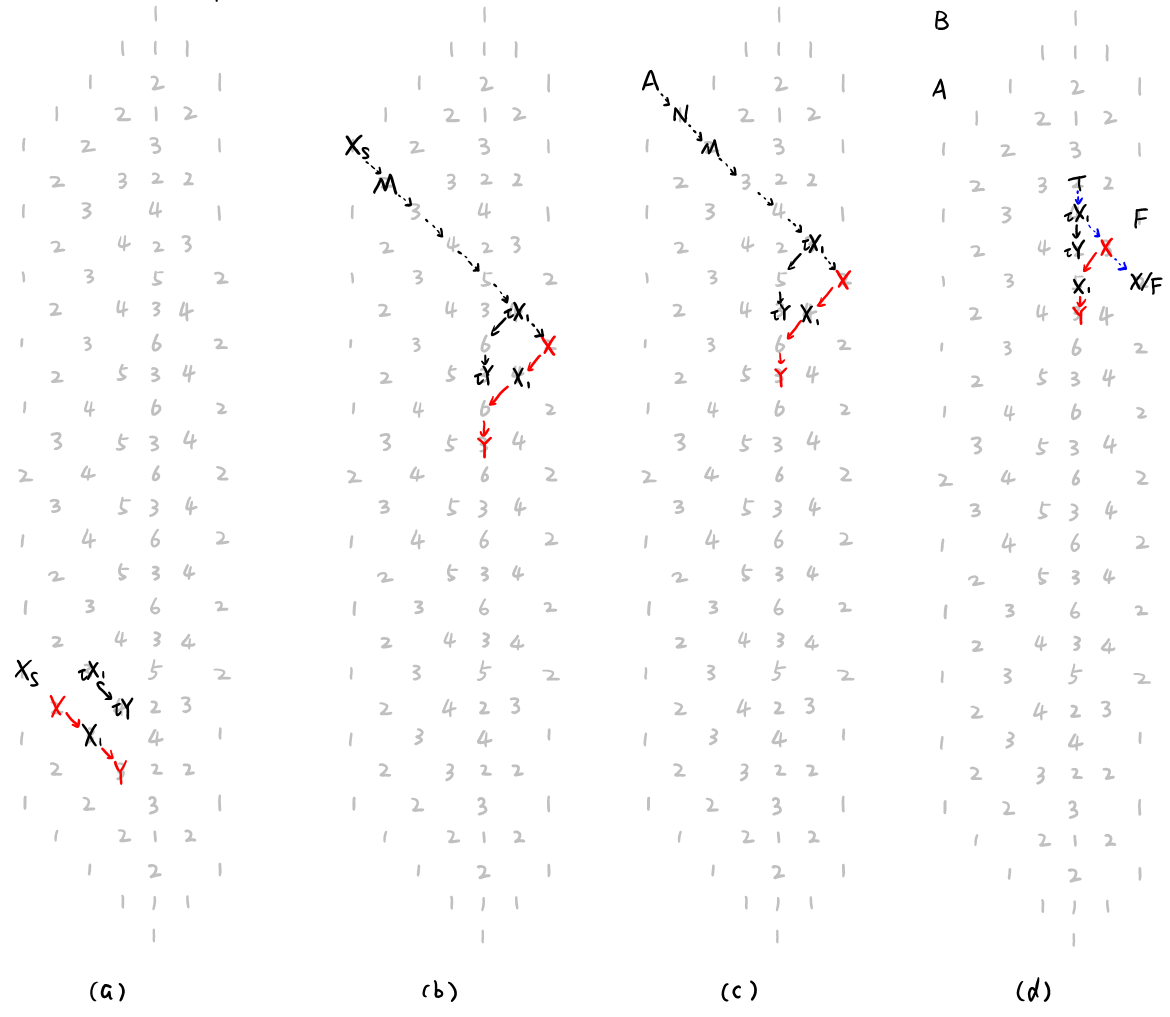
\includegraphics[width=7.5cm]{figures/specialcases.png}
	%		\captionsetup{labelformat=empty}
			\caption{special cases}
			\label{fig:specialcases}
			\vspace{0.2cm}
		\end{figure}
	\end{center}
\begin{eg}
In the case of Figure \ref{fig:specialcases}(a), if $X_1 \longrightarrow Y$ is injective, then
\begin{equation*}
\begin{aligned}
\Gr(Y) &\longrightarrow \Gr(X_1) \times \Gr(Y/X_1) \text{ or } U(X_1,X)\\
\Gr(X_1) &\longrightarrow \Gr(X) \times \Gr(X_1/X) \text{ or } U(X,X_S)\\
U(X_1,X) &\longrightarrow \Gr(X) \times \Gr(X_1/X) \\
U(X,X_S) &\longrightarrow \Gr(X_S) \times \Gr(X/X_S). \\
\end{aligned}
\end{equation*}

When $X_1 \longrightarrow Y$ is not injective, we get
$$\Gr(Y) \longrightarrow \Gr(X) \times \Gr(Y/X) \text{ or } U(X,X_S).$$
Since the map $\tau X_1 \longrightarrow \tau Y$ is injective, from Lemma \ref{lem:descriptionofX_S} we get $X_S\longrightarrow X$ is irreducible monomorphism. Thus
$$U(X,X_S) \longrightarrow \Gr(X_S) \times \Gr(X/X_S).$$
These maps give the variety $\Gr(Y)$ an affine paving from bottom to top.
\end{eg}
\begin{eg}
In Figure \ref{fig:specialcases}(b), we would like to prove that  $\Gr(Y)$ has the affine paving property. We have
$$\Gr(Y) \longrightarrow \Gr(X) \times \Gr(Y/X) \text{ or } U(X,X_S).$$
When the map $M \longrightarrow X$ is not monomorphism, we get
$$U(X,X_S) \longrightarrow \Gr(X_S) \times \Gr(X/X_S);$$
when the map $M \longrightarrow X$ is monomorphism, we get
\begin{equation*}
\begin{aligned}
U(X,X_S)&=U(X,M) \bigsqcup U(M,X_S)\\
U(X,M) &\longrightarrow \Gr(M) \times \Gr(X/M)\\
U(M,X_S) &\longrightarrow \Gr(X_S) \times \Gr(M/X_S).
\end{aligned}
\end{equation*}
Since the order of $X$, $Y/X$, $X_S$, $X/X_S$, $M$, $X/M$, $M/X_S$ are small or equal to $2$, the induction process stops, we get $\Gr(Y)$ has the affine paving property.
\end{eg}
\begin{eg}
In the case of Figure \ref{fig:specialcases}(c), we have 
$$\Gr(Y) \longrightarrow \Gr(X) \times \Gr(Y/X) \text{ or } U(X,X_S)$$
where $X_S=\ker(\tau X_1 \longrightarrow \tau Y)$. When $X_S=0$ we're done; if not, then $A \neq 0$ and $X_S=A$, we decompose $X_S \longrightarrow Y$ as compositions of minimal section monos:

Case 1: $M\longrightarrow X$ is not injective, then
 \begin{equation*}
 \begin{aligned}
 U(X,X_S)&=U(X,N) \bigsqcup U(N,X_S)\\
 U(X,N) &\longrightarrow \Gr(N) \times \Gr(X/N)\\
 U(N,X_S) &\longrightarrow \Gr(X_S) \times \Gr(N/X_S).
 \end{aligned}
 \end{equation*}
 
 Case 2: $M\longrightarrow X$ is injective, then
  \begin{equation*}
  \begin{aligned}
  U(X,X_S)&=U(X,M) \bigsqcup U(M,N) \bigsqcup U(N,X_S)\\
  U(X,M) &\longrightarrow \Gr(M) \times \Gr(X/M)\\
  U(M,N) &\longrightarrow \Gr(N) \times \Gr(M/N)\\
  U(N,X_S) &\longrightarrow \Gr(X_S) \times \Gr(N/X_S).
  \end{aligned}
  \end{equation*}
  
  Since $\Gr(X)$, $\Gr(Y/X)$, $\Gr(N)$, $\ldots$ have affine paving property, we conclude that $\Gr(Y)$ has also the affine paving property.
\end{eg}
\begin{eg}
Finally we begin to handle the most difficult case(Figure \ref{fig:specialcases}(d)). When $X \longrightarrow Y$ is not injective, we get
$$\Gr(Y) \longrightarrow \Gr(F) \times \Gr(Y/F) \text{ or } U(F,?)$$
then we get the result \footnote{$\Gr(F)$ is empty or a singleton, so is $U(F,?)$.}.

When $X \longrightarrow Y$ is injective, we have
$$\Gr(Y) \longrightarrow \Gr(X) \times \Gr(Y/X) \text{ or } U(X,X_S)$$
where $X_S=F\oplus \ker(\tau X_1 \longrightarrow \tau Y)=F \oplus T$ by Lemma \ref{lem:descriptionofX_S}. Since $X \longrightarrow Y$ is injective, we get $A=0$, thus $B=0$ also, and then the sectional map $T \longrightarrow X/F$ in injective. We thus get two short exact sequence satisfying the conditions in \ref{thm:main2}:
\begin{center}
% https://tikzcd.yichuanshen.de/#N4Igdg9gJgpgziAXAbVABwnAlgFyxMJZARgBoAGAXVJADcBDAGwFcYkRyQBfU9TXfIRQAmCtTpNW7AGLdeIDNjwEiAZjE0GLNohAANOXyWCiAFg0Tt7PQHpZPIwJUoArBa1TdnBwv7KhJKTE4h46HIa+xs7IbsGakmHe8opOAaJxlp4gACoRKf5qQSEJ1nZ5fiYo5hmhpXoA+gDK5VEB5O4lugA6XTA49Lo++ZXI7TWdID0AHliD4jBQAObwRKAAZgBOEAC2SG4gOBBIAOw+mzsnNIdIABxnW7uIN1dHiACc8VbdXWhYAOQRc6PD4HV4ANnuF0Q6lBSFMkMeolh0M+WR6v0BDyQZGRwgRSHayOIXEoXCAA
\begin{tikzcd}[row sep=0mm]
\eta: & 0 \arrow[r] & F \arrow[r] & X \arrow[r, "\pi"]    & X/F \arrow[r]   & 0 \\
\xi:  & 0 \arrow[r] & T \arrow[r] & X/F \arrow[r, "\pi'"] & X/X_S \arrow[r] & 0
\end{tikzcd}
\end{center}
Let $N \in \Gr(X)$ be a subrepresentation, it's obvious that $N \in \Gr(X_S) \iff \pi'\circ \pi(N)=0$, so 
  \begin{equation*}
  \begin{aligned}
  N\in U(X,X_S) & \iff \pi'\circ \pi(N) \neq 0\\
  & \iff \pi(N) \notin \Gr(T)\\
  & \iff \pi(N) \in U(X/F,T)\\
  & \iff \Psi_{\eta}(N) \in \Gr(F) \times U(X/F,T)
  \end{aligned}
  \end{equation*}
\end{eg}
Thus the Zarisky-locally trivial affine bundle map
$$U(X,F) \longrightarrow \Gr(F) \times \Gr(X/F)$$
restricted to the Zarisky-locally trivial affine bundle map
$$U(X,X_S) \longrightarrow \Gr(F) \times U(X/F,T).$$

Finally, by applying the short exact sequence $\xi$ to Theorem \ref{thm:main2} we get the map
$$U(X/F,T) \longrightarrow \Gr(X/F) \times \Gr(T).$$
Since all the Grassmannians $\Gr(X)$, $\Gr(Y/X)$, $\Gr(F)$, $\Gr(X/F)$, $\Gr(T)$ have the affine paving property, we conclude that $\Gr(Y)$ has the affine paving property.
\bibliographystyle{plain}
\bibliography{reference}





\end{document}




